\renewcommand{\lstlistingname}{Example}

The previous chapter covered the necessary background information on business process collaborations represented in BPMN and their different perspectives. In this chapter, the conception of the automatic process collaboration generator is introduced.

\section{Approach}

As already mentioned in Chapter \ref{chap:theo}, a process collaboration involving several partners can be modeled from different perspectives (partner or global) through the use of different model types. The process collaboration generator, implemented in the context of this work, generates all three different model types as the output. In general, there exist two different approaches to build a process collaboration with all the described models \cite{sabrina1174}. In the \textit{top-down approach}, first the choreography model is build, then the public and private models of each partner are derived and defined consistently. In comparison, in the \textit{bottom-up approach}, each partner has already defined a private and public process. Then, the choreography model is constructed by connecting the public models via message exchange. \par
The automatic generator, presented in this work, follows the \textit{top-down approach}, by first generating the choreography model and then deriving the collaboration, public and private models from it. Thereby, each interaction (choreography task) of the choreography model is converted into a send and receive task and then added to the involved partners processes, to build their public process models. In turn, each private model is derived from its corresponding public model by enriching the public model with abstract private tasks. The collaboration model is then built by composing the partner's public processes into one model.\\

\begin{wrapfigure}[11]{r}{0.5\textwidth}
\vspace{-0.5cm}
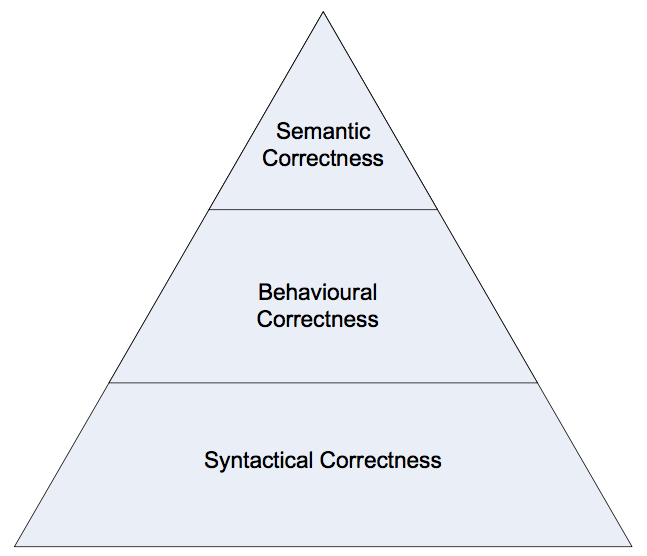
\includegraphics[width=0.9\linewidth]{src/images/correctness_levels.png}
\caption{Pyramid of Business Process Model Correctness\\(Source: \cite{sabrina848})}
\label{fig:bpm_correctness}
\end{wrapfigure}

Generally, when defining business process models, three levels of correctness need to be considered and satisfied by the models:\\

\textit{Syntactical Correctness} is defined by the underlying BPMN meta model and refers to the correct use and composition of the corresponding model elements. Syntactical constraints for example include the fact that any model must at least  have one start and one end event,\\ 
as well as  that flow  objects (e.g. tasks,\\ 
gateways, events) can only be connected\\
by control flow edges \cite{sabrina848}. \\

\textit{Behavioral Correctness} constitutes that a process model must be executable and therefore free of deadlocks or lifelocks. It assumes that the model is syntactically correct, because the behavior of a syntactical incorrect model is undefined. Regarding collaborative, cross-organizational processes, it is also required that the composition of the involved public models is compatible. For example, this means, that for every message that is send, a corresponding partner must be able to receive it \cite{sabrina1174, sabrina848}. \\

\textit{Semantic Correctness} means that the a process model must comply with imposed compliance rules \cite{sabrina848}. Thereby it must be differentiated between \textit{local} and \textit{global compliance rules}. \textit{Local compliance rules} constrain the private process of a partner, whereas \textit{global compliance rules} constrain the interaction between multiple partners \cite{sabrina1174}. In this work, only \textit{global compliance rules} are considered to constrain the choreography model.

\begin{figure}[H]
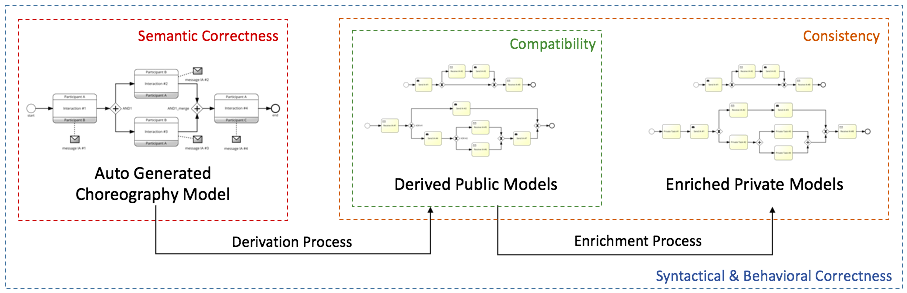
\includegraphics[width=1\textwidth]{src/images/conception_approach.png}
\caption{Top-Down Approach}
\label{fig:topdownapproach}
\end{figure}

All three correctness levels are considered by the proposed algorithm for implementing an automatic process generator. The algorithm ensures that only model specific flow objects are used to build the processes and that they are connected appropriately (syntactical correctness). It also guarantees the absence of deadlocks and lifelocks (behavioral correctness) and offers the possibility to define global compliance rules (see Chapter \ref{sec:conception_compliance}), to which the generated collaboration should comply (semantic correctness). Deriving all models from the before generated choreography model offers also the advantage, that if the deriving process is implemented correctly, it already ensures \textit{consistency} and \textit{compatibility} between the different models. In the context of collaborative processes, \textit{consistency} means, that the private model of a partner has to be consistent with the corresponding public model, whereas \textit{compatibility} requires the public models of the collaborating partners to be compatible with one another \cite{FDHILA20151}. This ensures that the executed business process of one partner satisfies the behavior that is communicated to the partners through his public models \cite{sabrina1174}. Figure \ref{fig:topdownapproach} illustrates the the collaboration generation approach with it's different levels of correctness.\\

\section{Constraining the Collaboration Generation} \label{sec:constraints}

Despite the premise that the process collaborations should be generated randomly, it is reasonable to set some boundaries within which the random generation takes place. The implemented generator provides two different ways to influence the resulting choreography model and hence the whole collaboration. The first one provides the possibility to constrain the choreography model in terms of the employed flow objects and their exact quantity by specifying several input parameters. The second one enables the user to impose global compliance rules based on compliance patterns to which the resulting model must comply.

\subsection{Parametric Constraints} \label{sec:param_constraints}

The following input parameters are specified to influence the random generation of the choreography model and hence also the deriving models:

\begin{itemize}
\item Number of Partners: \\Determines the number of participants that are involved in the process collaboration.
\item Number of Interactions: \\Determines the number of messages that are exchanged between the partners.
\item Number of Exclusive Gateways: \\Determines the number of Exclusive Gateways that are put into the model.
\item Number of Parallel Gateways: \\Determines the number of Parallel Gateways that are put into the model.
%\item Number of Loops: \\Determines the number of Loops that are put into the model.
\item Max. Branching: \\Determines the maximum possible number of paths created for each gateway.
\end{itemize}


%\textit{Number of Partners} determines the number of participants which are involved in the process collaboration, whereas \textit{Number of Interactions} specifies the number of messages which are exchanged between the partners. \textit{Number of Exlusive/Parallel Gateways} in combination with \textit{Max. Branching} influences the the branching of the resulting process model. The First applies the exact number of the respective flow object into the model, whereas the second sets the upper boundary of branching (splitting the path) for each gateway. The lower boundary is set to two. Within this range, the generating algorithm determines a random number of following paths for each gateway placed into the model. This is explained in more detail later one. \textit{Number of Loops} determines the exact number of loops that should be placed into the model.

\subsection{Compliance Constraints} \label{sec:conception_compliance}

Generally, compliance rules can be defined for different process flow perspectives of a process. It can be distinguished between compliance rules that constrain the control flow (sequence of activities), the data associated with the activities, the resources (specific user or role) that perform the activities or the time perspective. There exist several languages and approaches on how to define and specify compliance rules, including formal languages \cite{Ghose2007},\cite{GovMilSad:edoc:06:compliance}, visual languages \cite{sabrina953},\cite{Awad2008} and pattern-based approaches \cite{compliance_patterns}, \cite{Ramezani2012}. Both visual and pattern-based approaches aim at hiding formal details (e.g. temporal logic) and therefore simplifying the specification of compliance rules. \\

For the specification of compliance rules for the automatic process generator, the pattern-based approach of Turetken et. al. \cite{compliance_patterns} is utilized. In \cite{compliance_patterns} a repository of \textit{process control patterns} is introduced, which are high-level templates used to represent process properties which the process specification must satisfy. There are four different groups of patterns: 

\begin{itemize}
\item \textit{Order} patterns concern the sequencing of activities. For Instance, `\textit{Customer\_Inquiry} LeadsTo \textit{Offer}', is used to express that after an inquiry is sent and received, an offer must be sent at some point afterwards.
\item \textit{Occurrence} patterns represent rules that address the existence of certain activities. For instance, `\textit{Check\_Credit\_Worthiness} Universal', is used to express that the activity must always occur when the process is executed. 
\item \textit{Resource} patterns constrain that certain activities must be performed by a specific user or group of users (role). For instance, `\textit{Approve\_Offer} PerformedBy \textit{Role Q}' constrains, that the activity must be assigned to a user who is part of the user group Q.    
\item \textit{Time} patterns are used to assign temporal rules to Order or Occurrence patterns. For instance, `\textit{Customer\_Inquiry} LeadsTo \textit{Offer} Within \textit{7(days)}' constrains, that an Offer has to be replied within seven days after an inquiry has been received. 
\end{itemize}

Because the generated process collaborations neglect the data, time and resource perspective and focus solely on the control flow, only compliance rules that constrain the sequence of activities are possible to impose. Following process control patterns are supported to constrain the automatic generated choreography:

\begin{table}[H]
\centering
\resizebox{12cm}{!}
{
\begin{tabular}{l|l}
Pattern		      & Description  \\ \hline
P LeadsTo Q       & Interaction P must lead to Interaction Q	  	 \\
P Precedes Q      & Interaction Q must be preceded by Interaction P	  \\
P Universal  	  & Interaction P must always occur throughout execution \\
P Exists		  & Interaction P must be specified in process \\
\end{tabular}%
}
\caption{Overview of supported Compliance Patterns}
\label{tab:compl_patterns}
\end{table}

Note that the \textit{P LeadsTo Q} pattern does not demand an immediate succession of interaction Q on interaction P.


\section{Random Process Collaboration Generation}

In this chapter, the needed components and their functionality for implementing a random process generator are explained. Each component encapsulates a step of the above described approach. Based on this approach, four components with single responsibilities can be derived: one component is responsible for randomly generating a choreography model, one for imposing compliance rules on the resulting process, another for deriving the remaining model types and the last component keeps control over the overall process. In the following the components and their functionalities will be explained in details.

\subsection{Overall Process Controller} \label{sec:overallprocesscontroller}
The \textit{Overall Process Controller} represents the orchestration component for building random process collaborations, based on given constraints. The process follows the principle \textit{'first build then check'}, which means that after a random choreography model has been generated (see chapter \ref{sec:conChorGen}), it will then be checked if the interactions defined within the compliance rules, can be assigned into the already built model in such a way that the resulting interaction sequence complies to the imposed rules. If the interaction allocation is not possible without violating the compliance rules, new random models will be build until a compliant model has been generated. If the imposing of the compliance rules fails repeatedly, it's an indicator that the amount of interactions in the model is too small relative to the unique interactions specified within the compliance rules. To overcome this, the number of interactions is increased by 10 percent every 10th build. After a successful assignment of the compliance rules, the remaining public and private models are derived out of the generated choreography model. At last, all models will be translated into a valid BMPN/XML. The whole process of generating a random choreography by coordinating the different functions is outlined in Algorithm \ref{alg:choreographyController}. \\

\begin{algorithm}[H]
\small
\SetAlgoLined
buildSuccess = \textbf{false}\;
\While{buildSuccess $\neq$ \textbf{true}}{
	build new choreography model\;
	\eIf{compliance rules are defined}{
		assign interactions\;
		\uIf{assignment successful}{
			buildSuccess = \textbf{true}\;
		}\ElseIf{number of interaction $\bmod$ 10 $\equiv$ 0}{
			increase number of interactions by factor 1.1\;
		}

	}{
		buildSuccess = \textbf{true}\;
	}
}
generate whole collaboration\;
export models to BPMN\;
\caption{Overall Collaboration Generation Controller}
\label{alg:choreographyController}
\end{algorithm}

\subsection{Generating Random Choreography Models} \label{sec:conChorGen}
The actual algorithm for generating graphs, representing choreography models, is implemented within the \textit{Choreography Model Generator} component. Throughout the generation process, it is essential to keep track of the current model state at every point, in order to know where it is possible to put a new node without violating the syntactical and behavioral correctness of the resulting BPMN model. Therefore a \textit{Model Tracking} component is necessary, which provides control flow logic and a corresponding data model. The concept of this component is based on the RPST graph decomposition which was introduced by Vanathalo et al. in \cite{rpst}. In \cite{rpst}, a parsing algorithm for \textit{two-terminal graphs}\footnote{A directed graph that has a unique source node \textit{s} and a unique sink node \textit{t} $\neq$ \textit{s} with all other nodes \textit{V} are on a path from \textit{s} to \textit{t}.} is introduced that results in a unique graph decomposition represented as a hierarchical tree of \textit{modular} and \textit{objective fragments}. Modular means that a local change of the graph only impacts the corresponding, decomposed fragment, whereas objective requires that a fragment does not overlap with another fragment. Furthermore, fragments can be characterized as \textit{trivial} and \textit{non-trivial}. A fragment is \textit{trivial} if it contains exactly one edge and therefor, in the RPST, trivial fragments are represented by their edge and are always leaf nodes in the RPST. In contrast, each \textit{non-trivial} fragment is represented as non-leaf node. The root fragment (non-trivial) of a RPST decomposition contains all edges of a graph. Therefore it contains all other \textit{trivial} and \textit{non-trivial} fragments and has the source and sink node as it's boundaries. In the \textit{Model Tracking} component of this work, the equivalent of a modular and objective fragment is called a \textit{split}. A split is created for each gateway fork that is put into the model. Each split contains several \textit{branches} (minimum two and maximum is defined by the max\_branching parameter), that represent the different paths created by a parallel or exclusive gateway. Again, each branch holds the set of nodes that are on the path of a particular branch, whereas a path and therefore also a split, is limited by the merge node of its corresponding fork gateway node. In terms of a choreography model, nodes are limited to interactions and gateways. 

\begin{figure}[htb]
\centering
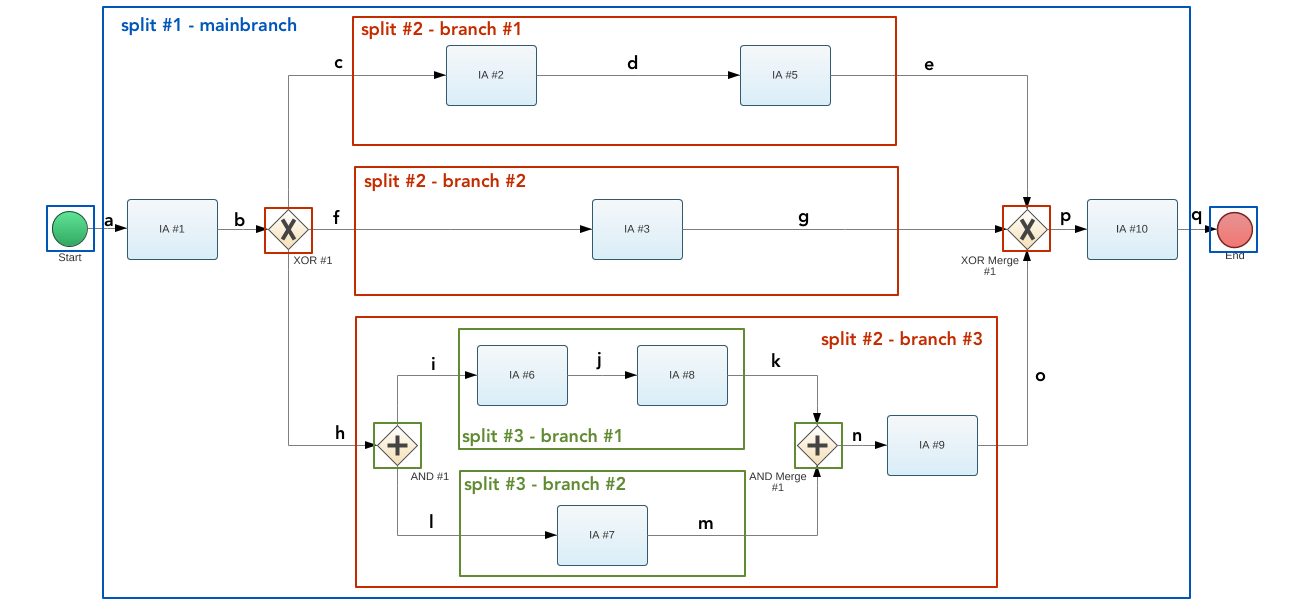
\includegraphics[width=0.9\textwidth]{src/images/graphTracking_1_edges.png}
\caption{Model Tracking Component - Concept}
\label{fig:graphTracking1}
\end{figure}

Figure \ref{fig:graphTracking1} illustrates the concept of this \textit{Model Tracking} component. In this example, there are in total three splits with the split nodes: start event (blue), exclusive gateway\#1 (red) and parallel gateway \#1 (green). The split with the start event as the split node and the end event as the merge node has always only one branch, the root branch. Technically, this is not a split in the sense of the terminology. But because of the underlying control flow logic and data model, which is shown in figure \ref{fig:graphTracking2}, that defines that every branch must be related to a split, this pseudo-split is necessary to keep track of the root branch.

\begin{figure}[htb]
\centering
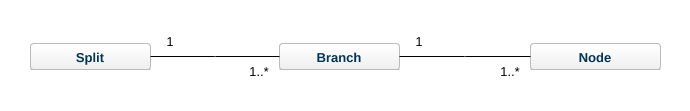
\includegraphics[width=0.8\textwidth]{src/images/graphtracking_dm.png}
\caption{Model Tracking Component - Data Model}
\label{fig:graphTracking2}
\end{figure}

The root branch (split \#1 - branch \#1) holds the set of ordered nodes: Interaction \#1, XOR gateway \#1, XOR merge \#1 and Interaction \#10. Split \#2 has three branches. The first branch contains the nodes Interaction \#2 and Interaction \#5. The second branch consists only of Interaction \#3 and the third branch contains AND gateway \#1, AND merge \#1 and Interaction \#9. At last, the third split consists of two branches, which hold the remaining interactions \#6, \#8 and \#7 respectively. Note that branches and therefore also splits, contain other splits, e.g. split \#2 contains split \#3 in branch \#3. This interleaving determines the hierarchy of the resulting RPST, which is shown in Figure \ref{fig:rpst_tree}. The root fragment is split \#1 and contains the non-trivial fragment \textit{split \#2} as well as the trivial fragments (edges) E = \{a, b, p, q\}. In turn \textit{split \#2} contains the non-trivial fragment \textit{split \#3} and the edges E = \{c, d, e, f, g, h, n, o\}. The last non-trivial fragment \textit{split \#3} contains the edges E = \{i, j, k, l, m\}.
\vspace{-0.25cm}
\begin{figure}[htb]
\centering
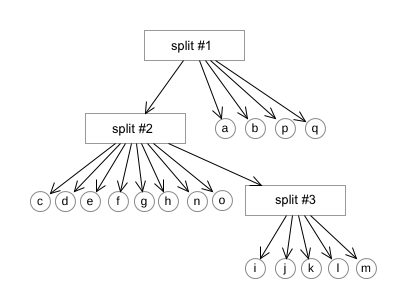
\includegraphics[width=0.6\linewidth]{src/images/graphTracking_rpst.png}
\caption{Refined Process Structure Tree}
\label{fig:rpst_tree}
\end{figure}

During the generation process, the current model build is maintained within the \textit{Model Tracking} component and simultaneously as a RPST graph. So far, there is no apparent necessity for the \textit{Model Tracking} component. But in order to automatically generate graphs representing choreography models, additional control flow logic is needed to ensure syntactically and behavioral correctness and to supervise the compliance with the build parameters. Therefor, each branch needs a status. This status indicates whether the branch is \textit{open}, \textit{splitted} or \textit{closed}. \textit{Open} defines, that the branch is not yet enclosed by the merge node of its corresponding split node and can further evolve by putting more nodes on its path. In turn, \textit{closed} defines that the branch is finalized and can not further evolve. Within the \textit{Model Tracking} component, a branch gets closed by putting the corresponding gateway merge node to the parent's branch and marking the branch as closed. Within the RPST graph, the merge node and an edge between the branch's last node with the merge node is added. A branch can also be in \textit{splitted} state, if it contains another split and none of this split's branches are yet closed, thus there exists no merge node for this split. In this case, a branch can not evolve until one of it's child split's branches is in state \textit{closed} and a merge node is placed on the branch. Then the state changes to \textit{open} again. For example, in figure \ref{fig:graphTracking3}, \textit{branch \#1} of \textit{split \#2} represents a branch in state \textit{split}, whereas the main branch is in state \textit{open} because \textit{branch \#2} of \textit{split \#1} is already closed by the merge node of \textit{split \#2}. When closing a branch, first it is necessary to determine if a branch is allowed to be closed, without violating the soundness of BPMN choreography models. This is dependent on the split node type of the branch. The premise is that if the split node type is a parallel gateway, the branch is determined as \textit{closable} only if there is an interaction on all its enclosed paths. This means, that if a branch has a child split, its not necessary that an interaction is on the parent branch itself but on the branches of its child split or even on a deeper nested branch.

\begin{figure}[htb]
\centering
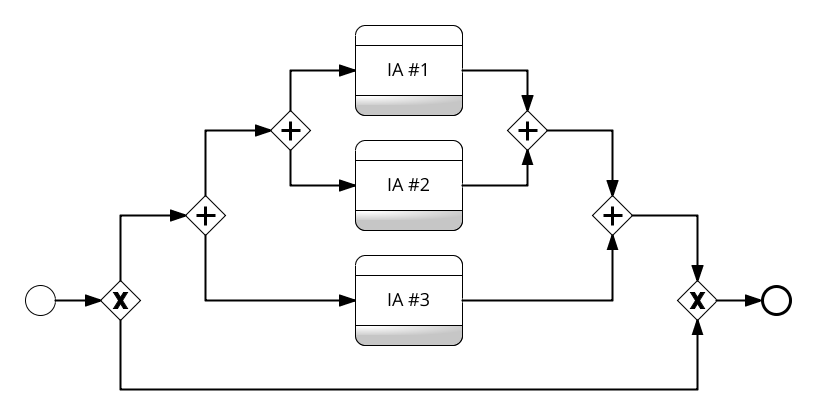
\includegraphics[width=0.7\textwidth]{src/images/choreo_min.png}
\caption{Minimum interactions reserved by remaining gateways}
\label{fig:graphTracking4}
\end{figure}
\vspace{-0.1cm}
For instance, see the upper branch of the second parallel gateway in Figure \ref{fig:graphTracking4}. The branch itself holds only another parallel gateway split node and a corresponding merge node but no interaction. This is valid because both branches of the parallel child split have an interaction and therefore also all enclosed paths of the parent branch. If the split node type is a exclusive gateway, it's allowed that one of the split's branches has no interaction on its path. For instance, see lowest branch of fist exclusive gateway in Figure \ref{fig:graphTracking4}. This depicts the circumstance that for an exclusive gateway, it's required to be able to also model a branch, where under certain process conditions no interaction between participants is necessary. This approach of tracking the status of the branches becomes crucial when only few remaining interactions are available and several branches are still open in the model. Because of the parametric limitation of the number of interactions, at a certain point in the build process or even directly in the beginning, if the proportion of specified gateways and interactions is small, interactions are not always allowed to be selected as next node type and not every open branch is allowed to be randomly selected for putting the next node into the model without resulting in a violation of the correctness of the model or exceeding the number of defined interactions. In order to determine whether this situation applies to a current point in a build process, the \textit{Model Tracking} component monitors the amount of \textit{free interactions} and \textit{reserved interactions}. 

Reserved interactions, are a subset of the remaining interaction that have either predetermined positions in the current graph (resInteractionsBranches) or will be needed in further paths created by not yet employed gateways (resInteractionsGateways). The exact amount of these reserved interactions depends on the number of non-closable branches of the current graph and the number of gateways that are not yet put into model. Regarding the current model, each open and non closable branch increases the amount of \textit{resInteractionsBranches} by one. Parallel gateways that are not yet placed into the graph will later create at least two new branches, which then again need at least one interaction on each of it's paths. Considering that a gateway node is allowed to be immediately followed by another gateways node without an interaction in between, the minimum amount of \textit{resInteractionsAndGateways} is \textit{remainingAndGateways} + 1. This premise also influences the impact of remaining exclusive gateways on the number of \textit{resInteractionsGateways}. Each remaining exclusive gateways only increases the number of \textit{resInteractionsGateways} by 1 if there is no more remaining parallel gateway. Because if there is also a remaining parallel gateway, the exclusive gateway could be put on a branch of the parallel gateway directly after the split and therefor the one needed interaction of the exclusive gateway is already considered in the calculation of \textit{resInteractionsAndGateways}. The influence of nested gateways onto the minimum amount of reserved interactions is illustrated in Figure \ref{fig:graphTracking4}. Given the parametric constraints \textit{numberOfInteractions = 3}, \textit{numberOfParallelGateways = 2} and \textit{numberOfExclusiveGateways = 1}, the figure represents one out of three possible resulting choreography models, which only differ in the sequence of used gateway types but not in the way of nesting and branching. After the amount of \textit{reserved interactions} is calculated, the number of \textit{free interactions} is determined by the difference between the amount of \textit{remaining interactions} and the number of \textit{reserved interactions}. Based on the values of the specified variables defined in Definition \ref{def:def1}, the node type of the next node to be put in the model and the corresponding position can be randomly selected without resulting in an incorrect model. For example, if the amount of \textit{free interactions} is $<$ 1, the random branch selection (position in the model) for putting the next node is limited to the branches that are not yet closable. On the other hand, if the amount of \textit{free interactions} $>$ 0, then all open branches can be selected for putting the next node. For the limitation of random branch selection, see also Algorithm \ref{alg:randBranch} and  Figure \ref{fig:graphTracking3}, which shows an unfinished choreography model at the point during the build process, assuming the parametric constrains numberOfInteractions = 6, numberOfAndGateways = 1 and numberOfExclusiveGateways = 1, where not all open branches are allowed to be selected for placing the node (in this case an interaction). In order to obtain a sound choreography model while not increasing the number of initially specified interactions, the sixth interaction is only allowed to be placed on branch \#2 of split \#3. In this scenario, \textit{reservedInteractionsTotal} equals one and \textit{freeInteractions} therefor equals zero. On the other hand, if assuming the total number of interactions being 7, all branches of split \#3 and the root branch are possible candidates for placing the sixth interaction, because at this point, \textit{freeInteractions} would equal one. In case of selecting the next possible node type, interactions are only allowed to be randomly selected, if the the amount of \textit{free interactions} $>$ 0 or not all remaining interactions are reserved by not yet consumed gateways.

\begin{Def}
	Let $x$ be the number of branches which are open and non-closable, \\$remainingInteractions$, all interactions not yet put into the model and \\$remainingXOR$ and $remainingAND$ the number of gateways not yet put into the model. Then
	\begin{center}
		\textbf{resInteractionsBranches} = x\\
		\textbf{resInteractionsAndGateways} = $remainingAND$ + 1\\
		\textbf{resInteractionsXORGateways} = \textbf{If} $remainingAND$ \textbf{$>$} 0 \textbf{Then} 0 \textbf{Else} 1\\
		\textbf{resInteractionsGateways} = $resInteractionsAndGateways$ + $resInteractionsXORGateways$\\
		\textbf{resInteractionsTotal} = $resInteractionsBranches$ + $resInteractionsGateways$\\
		\textbf{freeInteractions} = $remainingInteractions$ - $resInteractionsTotal$
	\end{center}
	\label{def:def1}
\end{Def}


\begin{figure}[]
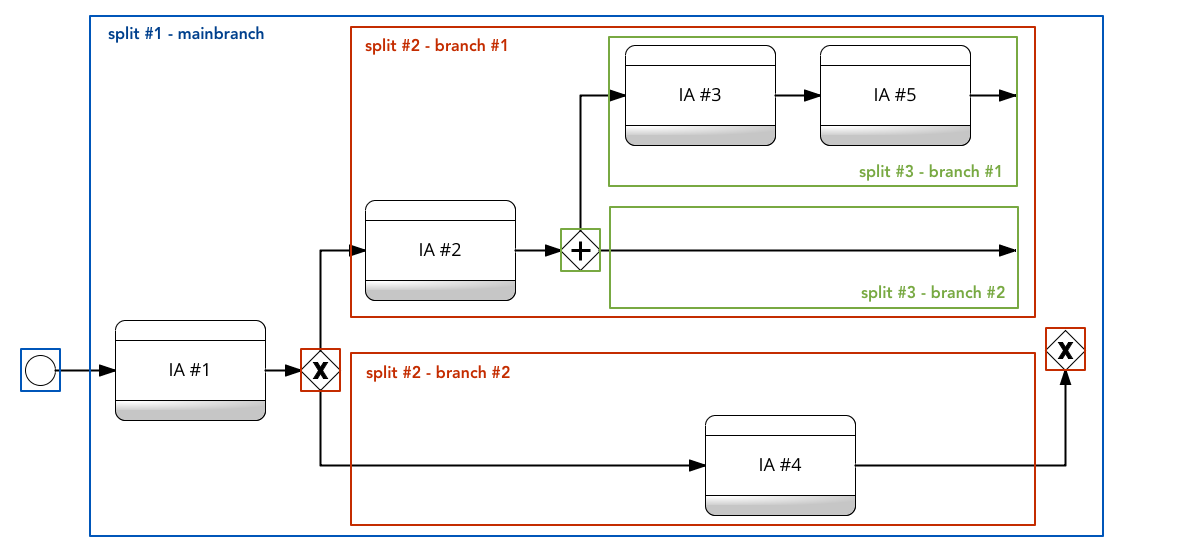
\includegraphics[width=1\textwidth]{src/images/choreo_branch_status.png}
\caption{Limitation of random branch selection}
\label{fig:graphTracking3}
\end{figure}
\vspace{-0.25cm}
The overall procedure of generating random choreography models is shown in Algorithm \ref{alg:choreoGen}. The input for a random model generation are the parametric constraints introduced in section \ref{sec:param_constraints}. At first, it is checked if the specified combination of the amount of interactions and gateways are sufficient for generating a sound model. This is the same evaluation as in determining the reserved interactions by remaining gateways. Therefore, the specified \textit{numberOfInteractions} must be greater or equal \textit{resInteractionsGateways}. If the validation is successful, the \textit{Model Tracking} component gets instantiated. Thereby, a split for the start event and the root branch is created. After this setup, the algorithm loops over the number of remaining interactions until all interactions are put into the model. Within each loop, at first a node type for the next node is randomly selected out of the pool of remaining nodes. This can be an interaction, exclusive or parallel gateway, depending on the number of free and reserved interactions as already explained. The algorithm for random possible node type selection is shown in Algorithm \ref{alg:randNodeType}.\\

\begin{algorithm}[H]
\small
\DontPrintSemicolon
\SetAlgoLined
\Begin{
	possibleNodeTypes $\leftarrow$ \{\}\;
	\If{freeInteractions $>$ 0 $\lor$ remainingInteractions > resInteractionsGateways}{
		possibleNodeTypes $\leftarrow$ possibleNodeTypes $\cup$ Interaction\;
	}
	\If{remainingParallelGateways $>$ 0}{
		possibleNodeTypes $\leftarrow$ possibleNodeTypes $\cup$ ParallelGateways\;
	}
	\If{remainingExclusiveGateways $>$ 0}{
		possibleNodeTypes $\leftarrow$ possibleNodeTypes $\cup$ ExclusiveGateways\;
	}
	\Return random NodeType of possibleNodeTypes\;	
}
\caption{getRandomNodeType()}
\label{alg:randNodeType}
\end{algorithm}
\vspace{0.4cm}
After a node type has been randomly selected, a position in the model is determined for placing a node of the previously selected node type by randomly selecting a possible open branch. Which branches are in the pool of possible, selectable branches, is again depending on whether there are free interactions available or not. If there are free interactions left, all open branches are allowed to be selected, independent of the priorly selected node type. Otherwise, only branches that are not closable are allowed to be included in the pool of possible branches. The algorithm for random possible branch selection is shown in Algorithm \ref{alg:randBranch}.\\

\begin{algorithm}[H]
\small
\DontPrintSemicolon
\SetAlgoLined
\Begin{
	possibleBranches $\leftarrow$ \{\}\;
	\eIf{freeInteractions $>$ 0 }{
		possibleBranches $\leftarrow$ all open branches\;
	}{
		possibleBranches $\leftarrow$ all not closable branches\;
	}
	\Return random Branch of possibleBranches\;	
}
\caption{getRandomBranch()}
\label{alg:randBranch}
\end{algorithm}
\vspace{0.4cm}
In the next step, the randomly selected branch is checked whether it's closable or not and if so gets closed by random. This doesn't apply to the root branch to make sure that there is always one branch where the model can further evolve. This step of random branch closing is necessary to obtain balanced choreography models regarding nested branches. If there would be no random branch closing mechanism, the resulting models would be very similar. A mechanism that closes branches whenever they are possible to close would only result in models with lesser nested branches whereas a mechanism that never closes branches would result in models that have highly nested branching. If the selected branch gets randomly closed, a merge node for the selected branch's split is created and added to the parent branch. Additionally, in the data model of the corresponding split, the merge node gets noted in order to assure that the last nodes of the other branches of this split will get connected with the same merge node as soon as they get closed. Finally, the algorithm jumps back to the beginning of the loop and starts again with randomly selecting a possible node type for the next node to be placed in the model.\\

\begin{algorithm}[H]
\small
\DontPrintSemicolon
\SetAlgoLined
\SetKwInOut{Input}{Input}\SetKwInOut{Output}{Output}
\Input{ 
\begin{itemize}[label={--}]
\setlength\itemsep{0em}
\item $minBranching \leftarrow$ 2\;
\item $maxBranching \leftarrow$ user specified upper branch amount border\;
\item $freeInteractions \leftarrow$ number of currently free interactions
\end{itemize}
}
\Begin{
	\eIf{freeInteractions $\geq$ 0}{
		$currentMaxBranching \leftarrow minBranching + freeInteractions$\;
		\If{currentMaxBranching $>$ maxBranching}{
			$currentMaxBranching \leftarrow maxBranching$\;
		}
	}{
		$currentMaxBranching \leftarrow minBranching$\;
	}
	
	\Return random value between $minBranching$ and $currentMaxBranching$\;	
}
\caption{getRandomBranchAmount()}
\label{alg:randBranchAmount}
\end{algorithm}
\vspace{0.5cm}
By the time a branch is not randomly closed, a node of the predefined node type gets instantiated. In case of an interaction, only the plain object without any sender, receiver or message gets instantiated. Is the selected node type a gateway, the number of branches is determined by randomly selecting a number between 2 and the current maximum branching amount. The maximum branching amount is generally limited by the user specified max branching parameter. But again, due to the limitation of interactions, the specified maximum amount of branches can not be adducted as the upper border without considering the current amount of free interactions. If only the user specified upper branching border (max. branching parameter) is adducted, there is a high chance that this would result in an inconsistent model, because the remaining interactions are insufficient for all paths created. In order to prevent this, the possible upper limit is determined dynamically each time a gateway node is put into the model by taking the minimum branching amount, which is always two, and adding the amount of free interactions. The algorithm for random possible branch amount selection is shown in Algorithm \ref{alg:randBranchAmount}. After a random number of branches is determined, the gateway node is added to the assigned branch and the corresponding split and branches are instantiated within \textit{Model Tracking}. Finally, the amount of the selected node type is decreased by one and the newly created edge between the preceding and the new node gets added into the RPST graph, before the loop starts over by selecting a random node type for the next node to be put into the model.\\

\begin{algorithm}[H]
\small
\DontPrintSemicolon
\SetAlgoLined
\SetKwInOut{Input}{Input}\SetKwInOut{Output}{Output}
\Input{ 
\begin{itemize}[label={--}]
\setlength\itemsep{0em}
\item $mainSplit \leftarrow$ split of root branch\;
\end{itemize}
}
\SetKwProg{Fn}{Function}{}{}
\Begin{
	\ForEach{branch of split.branches}{
		\ForEach{node of branch.nodes}{
			\If{node is gateway}{
				$closeSplit(split)$\;
			}
		}
		\If{branch is open}{
			$branch.close()$\;
		}
	}
}
\Fn{branch.close()}{
	$split \leftarrow$ split of branch\;
	\eIf{split.mergeNode == null}{
		$mergeNode \leftarrow$ instantiate merge node of gateway type\;
		$split.mergeNode \leftarrow$ mergeNode\;
		$branch.state \leftarrow$ closed\;
	}{
		$branch.state \leftarrow$ closed\;
	}
}
\caption{closeSplit(Split)}
\label{alg:finishModel}
\end{algorithm}
\vspace{0.5cm}
After all interactions and gateways are put into the model, the loop ends and all still open branches are getting closed. Algorithm \ref{alg:finishModel} displays the function to close all yet open branches by looping the model recursively. At this point, where the model doesn't further evolve, a branch is closed if the belonging split has a merge node assigned. If this is not the case, a merge node is created, added to the corresponding branch and assigned to the split.\\

\begin{algorithm}{hbt}
\small
\DontPrintSemicolon
\SetAlgoLined
\SetKwInOut{Input}{Input}\SetKwInOut{Output}{Output}
\Input{ 
\begin{itemize}[label={--}]
\setlength\itemsep{0em}
\item $remainingNodes \leftarrow$ number of nodes by type
\item $participants \leftarrow$ number of participants
\item $loops \leftarrow$ number of loops
\item $graph \leftarrow$ RPST graph
\end{itemize}
}
\SetKwProg{Fn}{Function}{}{}
\SetKw{Continue}{continue}
\Begin{
	\If{number of interactions $\leq$ number of gateways + 1}{
		model generation not possible\;
	}
	$modelTracking \leftarrow$ initialize model tracking component\;
	\While{$remainingInteractions > 0$}{ 
		$nextNodeType \leftarrow$ getRandomNodeType()\;
		$selectedBranch \leftarrow$ getRandomBranch()\;
		$precedingNode \leftarrow$ last node of $selectedBranch$\;
		\If{$precedingNode$ is $NULL$}{
			$precedingNode \leftarrow$ split node of $selectedBranch$\;
		}
		\eIf{$selectedBranch$ is closable}{
			close branch by random\;
			\If{closed}{
				\Continue
			}
		}{
			$nextNode \leftarrow$ instantiate node of $nextNodeType$\;
			\If{$nextNodeType$ is Gateway}{
				$branchCount \leftarrow$ getRandomBranchCount()\;
				$split \leftarrow$ instantiate new split\;
				$modelTracking.splits \leftarrow$ split\; 
				\For{$i \leftarrow$ 0 $branchCount$}{
					$branch \leftarrow$ instantiate new branch\;
					$split.branches \leftarrow branch$\;
					$i \leftarrow i$ + 1\;
				}
			}
			$selectedBranch.nodes \leftarrow$ $selectedBranch.nodes \cup nextNode$\;
			decrease $remainingNodes$ of $nextNodeType$\;
			add edge between $precedingNode$ and $nextNode$ to $graph$\;
		}
	}
	close still open splits\;
	add end event to root branch\;
	enrich interactions with reasonable sender and receiver sequence\;
}
\caption{Generate Choreography Model}
\label{alg:choreoGen}
\end{algorithm}

At this point the generated model is already syntactically correct because all model elements are used and connected according to BPMN specification. To achieve also behavioral correctness in choreography models, beside a correct sequence flow, a message flow must be incorporated. Therefore, a sender and receiver must be assigned to each interaction in order to form a valid sender-receiver sequence. Thereby, the sender of a succeeding interaction Q must always be either the sender or receiver of the directly preceding interaction P on the path. If this rule is not considered and the sender of a directly succeeding interaction Q is neither the sending nor the receiving participant of the directly preceding interaction P, a flawless execution of the process is not possible, because the sender of interaction Q will never know if the directly preceding interaction P has been performed yet. In case of gateways, additionally it is ensured that the receiver of the last interaction of each branch of the gateway is the same in order to determine a possible common sender for the succeeding interaction after the merge. Figure \ref{fig:messageFlow} illustrates a correct message flow within choreography models.  

\begin{figure}[htp]
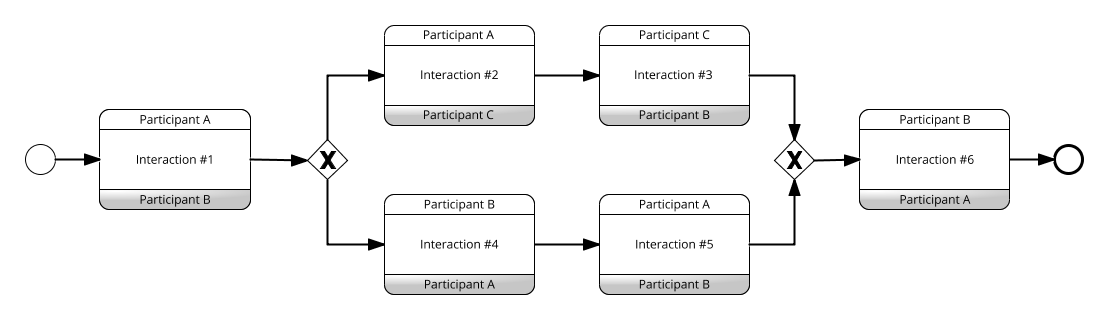
\includegraphics[width=1\textwidth]{src/images/messageFlow.png}
\caption{Message Flow - Sender/Receiver sequence}
\label{fig:messageFlow}
\end{figure}

Note that because of the fact that the sequence flow is first build without considering the corresponding message flow, it is likely that at some points an additional interaction must be inserted into the model to satisfy the above stated rules of sender-receiver sequences.

\subsection{Compliance Rules Assignment}
As pointed out in Chapter \ref{sec:overallprocesscontroller}, first a model is generated and afterwards it is checked whether the interaction sequence specified within the compliance rules can be applied to the generated model. Instead of considering the imposed compliance rule during the choreography generating, the followed approach was favored to allow users to specify compliance rules, which then can be imposed to also already existing choreography models in order to check if this particular model complies to the specified rules. Until now, the generated model complies only to the parametric constraints. The logic of specifying and imposing compliance rules is implemented within the \textit{Compliance Controller} component.\\

When specifying compliance rules to which the choreography model must comply, it must be checked whether the imposed rules are consistent with one another. In the context of the four supported patterns (see Table \ref{tab:compl_patterns}), this applies only to the two order patterns (LeadsTo and Precedes). For instance, consider the following set of compliance rules:

\begin{itemize}
\item \textit{CR-1}: P LeadsTo Q
\item \textit{CR-2}: Q LeadsTo S
\item \textit{CR-3}: S Precedes P
\end{itemize}

In this example, the rule \textit{CR-1} in combination with \textit{CR-2} is in conflict with \textit{CR-3}, because \textit{CR-1} and \textit{CR-2} determine, that the involved activities must occur in the order P-Q-S, whereas \textit{CR-3} constrains, that activity S must occur before activity P, which is in violation of the order determined by \textit{CR-1} and \textit{CR-2}. Algorithm \ref{alg:conflictCheck} shows the conflict checking procedure implemented within the \textit{Compliance Controller}. \\

\begin{algorithm}[H]
\small
\DontPrintSemicolon
\SetAlgoLined
\SetKwInOut{Input}{Input}
\SetKwInOut{Output}{Output}
\Input{ 
\begin{itemize}[label={--}]
\item compliance rule $cr$
\item dictionary $orderDependencies$ consisting of Interactions $P$ and their succeeding Interactions $S$
\end{itemize}
}
\SetKwProg{Fn}{Function}{}{}
\Begin{
	\If{$cr$ is order pattern}{
		$p \leftarrow$ preceding interaction of $cr$\;
		$s \leftarrow$ succeeding interaction of $cr$\;
		\eIf{!orderConflictCheck($p, s$)}{
			add $cr$ to $complianceRules$\;
			\eIf{$p \in P$ of $orderDependencies$}{
				add $s$ to succeeding interactions $S$ of $p$
			}{
				add $p$ to $orderDependencies$\;
				add $s$ to succeeding interactions $S$ of $p$ 
			}	
		}{
			add $cr$ to $conflictedRules$\;
		}
	}	
}
\Fn{orderConflictCheck($p, s$)}{
	\eIf{$s \in P$ of $orderDependencies$}{
		\ForEach{$s \in S$ of $p$}{
			\uIf{$s$ == $p$}{
				\Return \textbf{true}
			}\uElseIf{orderConflictCheck($s, p$)}{
				\Return \textbf{true}
			}
		}
	}{
		\Return \textbf{false} 	
	}
}
\caption{Adding Compliance Rules}
\label{alg:conflictCheck}
\end{algorithm}
\vspace{0.5cm}
The result of this procedure is a set of conflict free compliance rules, which determines a specific order sequence between the involved interactions. The specific interactions of the compliance rules are then eventually assigned to the existing interactions within the before generated model in a way that it complies to the interaction order and the compliance rules. Therefore, the first step is to determine all possible positions within the model for each compliance rule. The result is a set of possible position combinations (interactions placed in the model during initial choreography generation) for the compliance rule specified Interaction P and Interaction Q. For each possible position of Interaction P there has to be at least one possible position for Interaction Q. The rules that determine applicable positions for the four implemented compliance patterns are shown in Definitions \ref{def:leadsto} - \ref{def:exists}. \\

The difference between the determination of possible positions for the patterns \textit{LeadsTo} and \textit{Precedes} is that in case of \textit{P LeadsTo Q} the position for Interaction Q must always be reached after the position of Interaction P has been reached, whereas in case of \textit{P Precedes Q} the Interaction Q must only be possible to reach afterwards. In other words, if Interaction Q is executed, Interaction P must have occurred before. This means that unlike for the \textit{LeadsTo} pattern, in case of a \textit{Precedes} the succeeding interaction Q can also be inside an exclusive branch of the subsequent path of interaction P. For example, let P be assigned to \textit{Interaction IA 2} of the choreography model shown in figure \ref{fig:crassign}. In case of a \textit{Precedes} pattern, the set of possible interactions for Q is \textit{Q}\textsubscript{IA2} = \{IA 3, IA 4, IA 5, IA 6, IA 7, IA 8, IA 9, IA 10, IA 11, IA 12, IA 13, IA 14\}. These are all interactions that are possibly reachable after IA 2 has been reached. On the other hand, in case of \textit{LeadsTo}, the set of possible interaction assignments \textit{Q}\textsubscript{IA2} only includes \{IA 13, IA 14\}, because if IA 2 has been reached, only these two are always possible to be reached afterwards. Additionally to this rules, for a given P assigned within a parallel branch, the succeeding interaction Q is not allowed to be assigned to a position of another parallel branch, because there is no control mechanism that ensures the correct sequence of parallel interactions. This must be considered for both order patterns.

\begin{Def}
	Possible position assignments for the interactions P and Q of a compliance pattern P LeadsTo Q are as following:
	\begin{center}
		\textbf{Interaction P} = An interaction that has interactions on its subsequent paths that will always be reached.\\
		\textbf{Interaction Q} = An interaction that will always be reached after Interaction P has been reached.\\
	\end{center}
	\label{def:leadsto}
\end{Def}

\begin{Def}
	Possible position assignments for the interactions P and Q of a compliance pattern P Precedes Q are as following:
	\begin{center}
		\textbf{Interaction P} = An interaction that is always reached prior to Interaction Q.\\
		\textbf{Interaction Q} = An interaction that has interactions on its preceding path that were always reached prior to Interaction Q.\\
	\end{center}
	\label{def:precedes}
\end{Def}

The two occurrence patterns \textit{Universal} and \textit{Exists} differ only in that in for \textit{P Universal}, the position of interaction P must always be reached throughout process execution, whereas for \textit{P Exists} the position of interaction must only be reachable or in other words must be defined within the model.

\begin{Def}
	Possible position assignments for the interaction P of a compliance pattern P Universal are as following:
	\begin{center}
		\textbf{Interaction P} = An interaction that will always be reached.\\
	\end{center}
	\label{def:universal}
\end{Def}

\begin{Def}
	Possible position assignments for the interaction P of a compliance pattern P Exists are as following:
	\begin{center}
		\textbf{Interaction P} = An interaction that can be reached.\\
	\end{center}
	\label{def:exists}
\end{Def}

\begin{figure}[H]
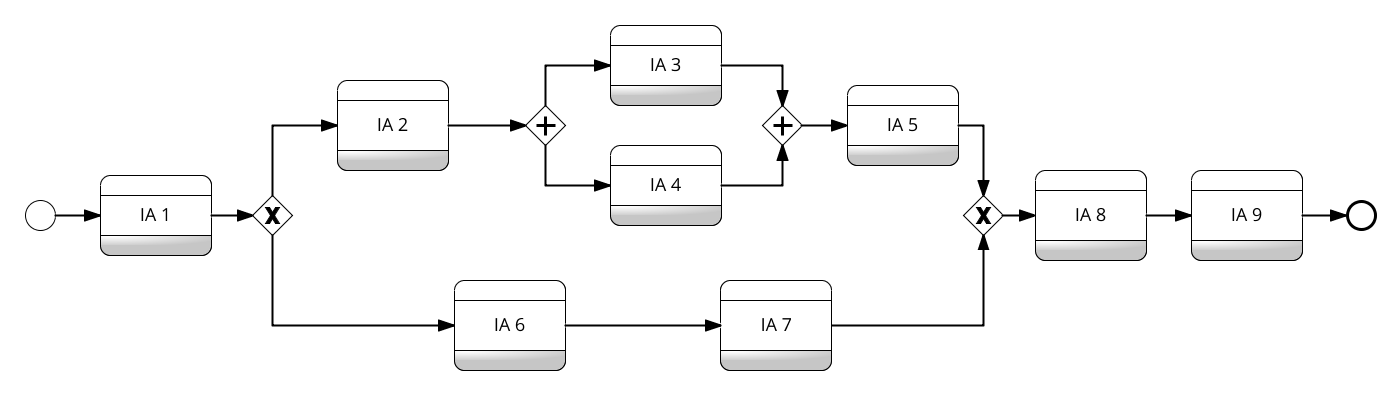
\includegraphics[width=1\textwidth]{src/images/cr_assign.png}
\caption{Compliance Rule Assignment}
\label{fig:crassign}
\end{figure}

If the interactions used for specifying the rules are disjoint between all the compliance rules, the sets of assignment combinations are already sufficient to assign the involved interactions to positions that result in a model that is compliant with the opposed rules. But if there are particular interactions that are used in more than one compliance rule specification, the intersection of the interaction's possible assignments of all involved compliance rules represents the set of possible assignments for this particular interaction. For example, consider the choreography model shown in Figure \ref{fig:crassign} and the following compliance rules within which interaction B and C are each specified in the compliance rules \textit{CR-1} and \textit{CR-2}:

\begin{itemize}
\item \textit{CR-1}: Interaction A LeadsTo Interaction B
\item \textit{CR-2}: Interaction C Precedes Interaction B
\item \textit{CR-3}: Universal Interaction C
\end{itemize}

The three compliance rules form two valid order sequences between the three specified interactions: Interaction A $\rightarrow$ Interaction C $\rightarrow$ Interaction B and Interaction C $\rightarrow$ Interaction A $\rightarrow$ Interaction B. More than one valid order indicates that there is no strict sequence between some defined interactions. For example, within the three stated compliance rules there is no determined sequence between \textit{Interaction A} and \textit{Interaction C}. Thus, that in this case, the two interactions can be also assigned to paths that are parallel to one another. If there is more than one possible order, the implemented procedure choses one by random.

\begin{algorithm}[hbt]
\small
\DontPrintSemicolon
\SetAlgoLined
\SetKwInOut{Input}{Input}\SetKwInOut{Output}{Output}
\Input{
	$interactionOrder \leftarrow$ ordered CR interactions\;
} 
\SetKwProg{Fn}{Function}{}{}
\SetKw{Continue}{continue}
\Begin{
	determinePossibleAssignments()\;
	\ForEach{interaction in interactionOrder}{
		\If{!assignInteraction(interaction)}{
			\Return \textbf{false}\;
		}
	}
}
\Fn{assignInteraction(Interaction ia)}{
	$affectedCRs \leftarrow$ all compliance rules with ia involved\;
	$crPossibleAssignments \leftarrow$ HashMap$<$cr, model interactions$>$\;
	$modelAssignments \leftarrow$ HashMap$<$cr interaction, model interaction$>$\;  
	\ForEach{cr in affectedCRs}{
		\uIf{ia is specified P of cr}{
			$crPossibleAssignments \leftarrow$ add all possible model interactions for P\;  
		}\uElseIf{ia is specified Q of cr}{
			$pAssignment \leftarrow$ already assigned model interaction of P
			$crPossibleAssignments \leftarrow$ add all possible model interactions of Q for the given P\; 
		}
	}
	$commonPossibleAssignments \leftarrow$ common model interactions between all crPossibleAssignment entires\;
	\eIf{commonPossibleAssignments is not empty}{
		$selectedInteraction \leftarrow$ get interaction with most succeeding interactions out of commonPossibleAssignments\;
		$modelAssignments \leftarrow$ add ia with selected model interaction\;
		\Return \textbf{true}\;
	}{
		\Return \textbf{false}\;
	}
}
\caption{Compliance Rules Assignment}
\label{alg:imposecr}
\end{algorithm}

After the interaction order is set, for every specified compliance rule the possible model positions are determined independently, based on the rules defined in Definitions \ref{def:leadsto} to \ref{def:exists}.  The result of this step is shown in Tables \ref{tbl:crAssignment1} to \ref{tbl:crAssignment3}. These two steps are the preconditions for the actual assignment of the interactions into the existing model, which is shown in Algorithm \ref{alg:imposecr}. The assignment procedure iterates over the interaction order and for each interaction the intersection of the possible assignments of all affected compliance rules (commonPossibleAssignments) is calculated. Is the current interaction specified as the succeeding interaction of an affected order compliance rule, the possible model positions of this rule are limited to the succeeding model positions of the corresponding, already assigned, preceding interaction. For instance, let the order of the example compliance rules be C $\rightarrow$ A $\rightarrow$ B and let \textit{Interaction C} be already assigned to \textit{IA 1} and \textit{Interaction A} to \textit{IA 3} of the model shown in Figure \ref{fig:crassign}. In order to determine the possible model positions for \textit{Interaction B}, the intersection of the sets of possible positions for \textit{Interaction B} of the affected rules \textit{CR-1} and \textit{CR-2} has to be determined: 

\begin{itemize}
\item \textit{CR-1}: \{IA5, IA8, IA9\}
\item \textit{CR-2}: \{IA2, IA3, IA4, IA5, IA6, IA7, IA8, IA9\}
\item \textit{CR-1 $\cap$ CR-2}: \{IA5, IA8, IA9\}
\end{itemize}

Is the resulting intersection of the sets of possible assignments empty, then there is no valid position in the model where the interaction could be assigned to. In this case, the whole assignment process fails and results in a failed choreography build process, which triggers a new build process from the beginning (see Algorithm \ref{alg:choreographyController} - line 6). Is the intersection of possible model positions not empty, the procedure choses the interaction that has the most interactions on it's succeeding path, or in terms of RPST, the highest ranked trivial fragment on the hierarchy. This ensures, that the assignment process does not fail because of higher ranked interactions being assigned to positions at the end of the model, so that there are no valid positions left for lower ranked ones.  

\begin{table}[H]
\centering
\begin{tabular}{ll}
\multicolumn{1}{l|}{Interaction A}    & Interaction B                \\ \hline
\multicolumn{1}{l|}{IA1}  & \{IA8, IA9\}                      \\
\multicolumn{1}{l|}{IA2}  & \{IA3, IA4, IA5, IA8, IA9\}                           \\
\multicolumn{1}{l|}{IA3}  & \{IA5, IA8, IA9\} \\
\multicolumn{1}{l|}{IA4}  & \{IA5, IA8, IA9\}          \\
\multicolumn{1}{l|}{IA5}  & \{IA8, IA9\}                \\
\multicolumn{1}{l|}{IA6}  & \{IA7, IA8, IA9\}                 						\\
\multicolumn{1}{l|}{IA7}  & \{IA8, IA9\}                \\
\multicolumn{1}{l|}{IA8}  & \{IA9\}                     \\
\multicolumn{1}{l|}{IA9}  & \{\}               \\ \hline
\end{tabular}
\caption{Possible assignment combinations for CR-1}
\label{tbl:crAssignment1}
\end{table}

\begin{table}[H]
\centering
\begin{tabular}{ll}
\multicolumn{1}{l|}{Interaction C}    & Interaction B                \\ \hline
\multicolumn{1}{l|}{IA1}  & \{IA2, IA3, IA4, IA5, IA6, IA7, IA8, IA9\}                      \\
\multicolumn{1}{l|}{IA2}  & \{IA3, IA4, IA5\}                           \\
\multicolumn{1}{l|}{IA3}  & \{IA5\} \\
\multicolumn{1}{l|}{IA4}  & \{IA5\}          \\
\multicolumn{1}{l|}{IA5}  & \{\}                \\
\multicolumn{1}{l|}{IA6}  & \{IA7\}                     \\
\multicolumn{1}{l|}{IA7}  & \{\}                \\
\multicolumn{1}{l|}{IA8}  & \{IA9\}                     \\
\multicolumn{1}{l|}{IA9}  & \{\}               \\ \hline
\end{tabular}
\caption{Possible assignment combinations for CR-2}
\label{tbl:crAssignment2}
\end{table}


\begin{table}[H]
\centering
\begin{tabular}{l}
Interaction C \\ \hline
IA1 \\
IA8 \\
IA9 \\ \hline
\end{tabular}
\caption{Possible assignments for CR-3}
\label{tbl:crAssignment3}
\end{table}

\subsection{Deriving the Collaboration Models}

Following the introduced \textit{top-down approach}, the collaboration model as well as the public and private models of each partner are derived from the generated choreography model. As already mentioned, the public models are projections of the choreography model, which means that they represent the view on the collaboration process from the perspective of each involved participant, while focusing on the process of one participant at a time. They only include activities that are necessary to communicate with other process participants. The private models are then enhanced versions of the public models. Additionally, they include internal process activities that don't involve interaction with other participants and that are not relevant for other participants to know. At last, the collaboration model is the interconnection between the public models of each participant. Together they form a holistic view on the whole collaboration process and is therefore a different representation of the choreography model, without any information loss.\\
In the process of deriving the models, each interaction of the choreography model results in a send and receive task in the corresponding public models of the involved partners. In the public model of the initiating participant of an interaction, a send task is inserted and in the model of the receiving participant a corresponding receive task. Additionally, for each public model, it is tried to reduce the model's sequence flow as much as possible without violating the underlying, predetermined sequence flow of the choreography model. Thereby, each gateway of the choreography model is checked for interactions within its subsequent paths involving the current participant. If there are none, the gateway and it's subsequent paths are not put into the public model of this participant.\\  

\begin{figure}[H]
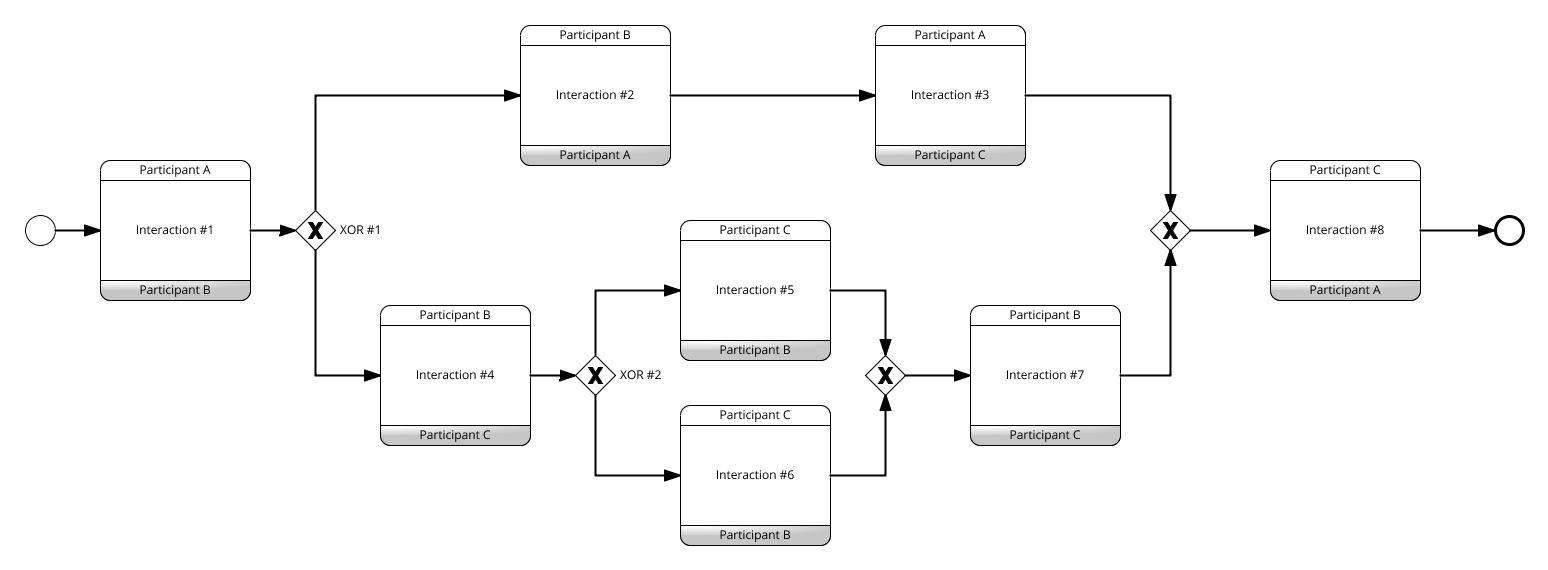
\includegraphics[width=1\textwidth]{src/images/choreo2public_choreo.png}
\caption{Choreography Model}
\label{fig:choreo2public}
\end{figure}

For instance, the choreography model shown in figure \ref{fig:choreo2public} would result in the three public models shown in Figures \ref{fig:choreo2public_pub} to \ref{fig:choreo2public_pub3}. The public model of Participant A (figure \ref{fig:choreo2public_pub}) is the only model where the sequence flow can be reduced in comparison to the choreography model. Because the lower path of the exclusive gateway \textit{XOR \#1} does not involve interactions that affect participant A, the whole path with all it's subsequent paths are not necessary and therefor not put into the public model.\\

\begin{figure}[H]
\centering
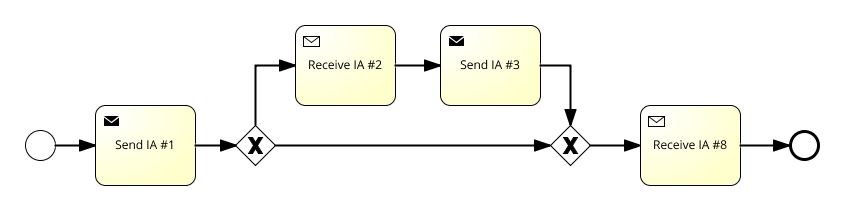
\includegraphics[width=0.8\textwidth]{src/images/choreo2public_pub1.png}
\caption{Public Model - Participant A}
\label{fig:choreo2public_pub}
\end{figure}

\begin{figure}[H]
\centering
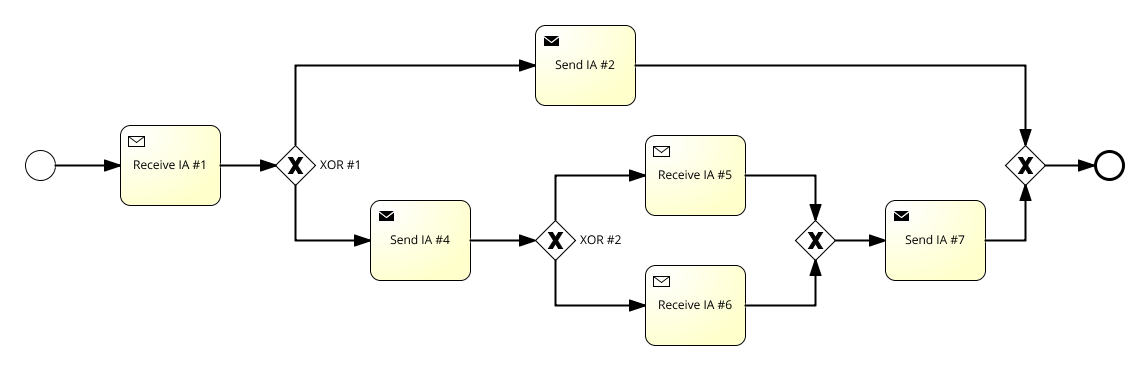
\includegraphics[width=0.8\textwidth]{src/images/choreo2public_pub2.png}
\caption{Public Model - Participant B}
\label{fig:choreo2public_pub2}
\end{figure}

\begin{figure}[H]
\centering
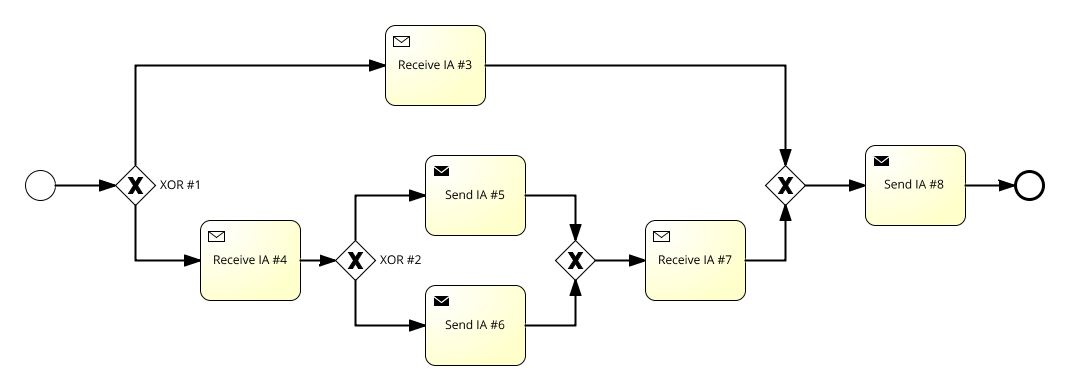
\includegraphics[width=0.8\textwidth]{src/images/choreo2public_pub3.png}
\caption{Public Model - Participant C}
\label{fig:choreo2public_pub3}
\end{figure}

In order to derive the private models from the public models, the public models are randomly enriched with private tasks, as well as some additional sequence flow elements (gateways) without violating the predefined sequence flow. The public models could also be used as private models without the enrichment, but because in real process scenarios, it is not likely that a participant does only perform public, interacting tasks, this enrichment is implemented. Figure \ref{fig:choreo2public_pr1} shows a possible outcome of a private model for participant A. 

\begin{figure}[H]
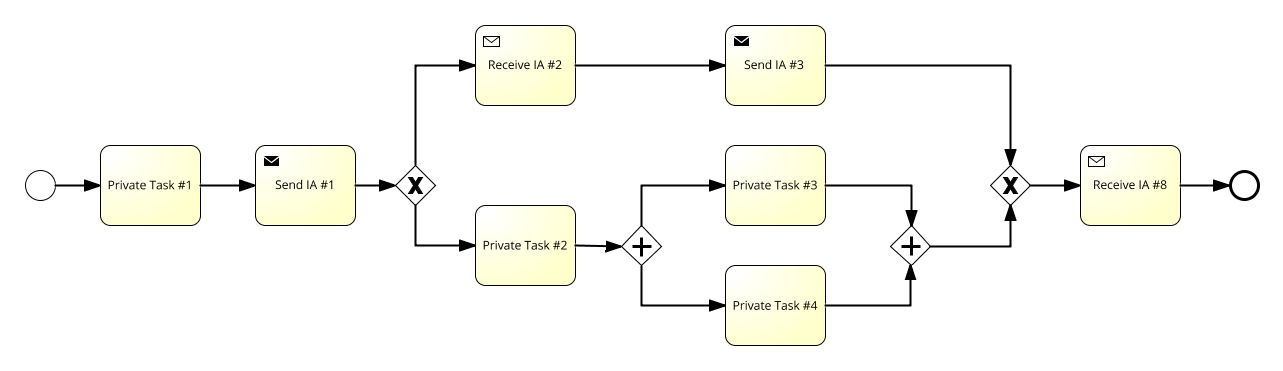
\includegraphics[width=1\textwidth]{src/images/choreo2public_pr1.png}
\caption{Possible Private Model - Participant A}
\label{fig:choreo2public_pr1}
\end{figure}

\section{Model Translation to BPMN/XML} \label{sec:bpmntranslation}
BPMN is the standard for describing business processes of any kind and therefore it is necessary to translate the generated process collaboration models in order to make them shareable and usable by a broad audience. Also, if some conventions are respected, the translated private models are out of the box executable and therefore the process can be tested by typical process engines. In order to translate the RPST representation of the models to BPMN/XML, the internal model elements for events, tasks, gateways, edges and participants must be mapped to the corresponding BPMN elements (see Table \ref{tab:flow_objects}) of the different model types and a process for generating a valid BPMN file must be designed. It has to be mentioned that the resulting BPMN/XML files only contain the formal process description. A generation of a the graphical process description will not take place. The following Table \ref{tbl:common2bpmn} shows the mapping of model type independent objects. These objects are used in all different model types and are therefore also common in the different BPMN models. Each model object is referenced by or has a reference to one or more other objects. For instance, the edges between flow objects do always refer to the flow objects (tasks and gateways) that are connected through this edge or, in case of an interaction, the message being sent is referenced. For this purpose, each model object has a unique id that also must be generated during the translation process.\\

\lstset{language=XML, morekeywords={definitions, encoding, xmlns, typeLanguage, targetNamespace, xsi:schemaLocation, message, id, name, choreography, isClosed, participant, messageFlow, messageRef, sourceRef, targetRef, choreographyTask, initiatingParticipantRef, incoming, outgoing, participantRef, messageFlowRef, startEvent, endEvent, parallelGateway, exclusiveGateway, gatewayDirection, sequenceFlow, sendTask, receiveTask, task}, basicstyle=\tiny, breaklines=true}

\begin{table}[H]
\centering
\begin{tabular}{l|l}
\multicolumn{1}{c|}{\textbf{Internal Object}} & \multicolumn{1}{l}{\textbf{BPMN/XML Element}}     \\ \hline
Participant &
\begin{lstlisting}
<participant id="(unique-id)" name="(name)"/>       
\end{lstlisting}\\ \hline
Start Event &
\begin{lstlisting}
<startEvent id="(unique-id)" name="">
  <outgoing>ref-to-sequenceFlow</outgoing>
</startEvent>       
\end{lstlisting} \\ \hline
End Event &
\begin{lstlisting}
<endEvent id="(unique-id)" name="">
  <incoming>ref-to-sequenceFlow</incoming>
</startEvent>       
\end{lstlisting} \\ \hline
Parallel Gateway &
\begin{lstlisting}
<parallelGateway id="(unique-id)" name="" 
  gatewayDirection="Diverging">
      <incoming>ref-to-sequenceFlow</incoming>
      <outgoing>ref-to-sequenceFlow</outgoing>
      <outgoing>ref-to-sequenceFlow</outgoing>
</parallelGateway>

<parallelGateway id="(unique-id)" name="" 
  gatewayDirection="Converging">
      <incoming>ref-to-sequenceFlow</incoming>
      <incoming>ref-to-sequenceFlow</incoming>
      <outgoing>ref-to-sequenceFlow</outgoing>
</parallelGateway>      
\end{lstlisting} \\ \hline
Exclusive Gateway &
\begin{lstlisting}
<exclusiveGateway id="(unique-id)" name="" 
  gatewayDirection="Diverging">
      <incoming>ref-to-sequenceFlow</incoming>
      <outgoing>ref-to-sequenceFlow</outgoing>
      <outgoing>ref-to-sequenceFlow</outgoing>
</exclusiveGateway>

<exclusiveGateway id="(unique-id)" name="" 
  gatewayDirection="Converging">
      <incoming>ref-to-sequenceFlow</incoming>
      <outgoing>ref-to-sequenceFlow</outgoing>
      <outgoing>ref-to-sequenceFlow</outgoing>
</exclusiveGateway>       
\end{lstlisting} \\ \hline
Edge & 
\begin{lstlisting}
<sequenceFlow id="(unique-id)" name="" 
  sourceRef="(ref-to-flow-object)" 
    targetRef="(ref-to-flow-object)"/>          
\end{lstlisting} \\ \hline
Message & 
\begin{lstlisting}
<message id="(unique-id)" name=""/>

<messageFlow id="(unique-id)" messageRef="(ref-to-message)" 
	sourceRef="(ref-to-sendTask/participant)" 
	targetRef="(ref-to-receiveTask/participant)"/>          
\end{lstlisting} \\ \hline
\end{tabular}
\caption{Mapping Common Model Elements to BPMN/XML}
\label{tbl:common2bpmn}
\end{table}

In the following, for each model type, the mapping of the internal model elements to the corresponding BPMN elements is explained. Because collaboration, public and private model share the same BPMN structure, they are consolidated in one chapter.

\subsection{Choreography Model}

The flow object interaction is the only unique object in choreography models. It references the connecting edges (sequenceFlows), the messageFlow and the two participants, that are interacting. Table \ref{tbl:choreo2bpmn} shows the structure of the corresponding BPMN/XML object. 
\\
\\
\begin{table}[H]
\centering
\begin{tabular}{l|l}
\multicolumn{1}{c|}{\textbf{Internal Object}} & \multicolumn{1}{l}{\textbf{BPMN/XML Element}}     \\ \hline
Interaction & 
\begin{lstlisting}
<choreographyTask id="" name="" initiatingParticipantRef="">
	<incoming>ref-to-sequenceFlow</incoming>
	<outgoing>ref-to-sequenceFlow</outgoing>
	<participantRef>ref-to-participant</participantRef>
	<participantRef>ref-to-participant</participantRef>
  	<messageFlowRef>ref-to-messageFlow</messageFlowRef>
</choreographyTask>
\end{lstlisting} \\ \hline
\end{tabular}
\caption{Mapping Choreography Model to BPMN/XML}
\label{tbl:choreo2bpmn}
\end{table}


\begin{figure}[H]
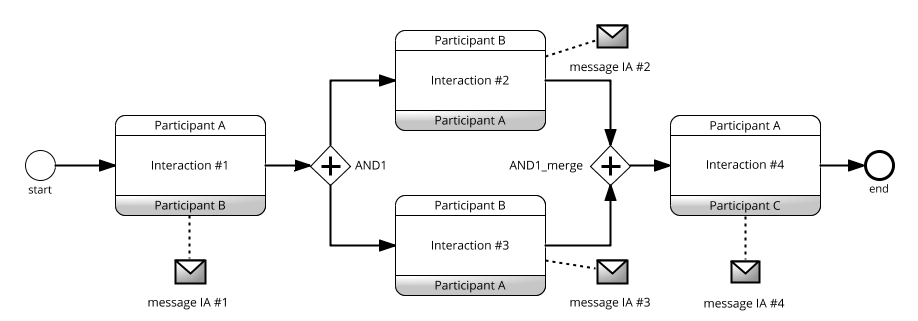
\includegraphics[width=1\textwidth]{src/images/choreo2bpmn.png}
\caption{BPMN/XML Translation Example - Choreography Model}
\label{fig:choreo2bpmn}
\end{figure}

The BPMN/XML shown in Example \ref{lst:choreobpmnex} represents the valid translation of the example choreography model shown in Figure \ref{fig:choreo2bpmn}. Independent from the model type, every BPMN/XML has the root element \textit{definitions} with the namespace and schema declarations. The actual model objects are located inside the \textit{choreography} element as already explained above. Because all different model types share a common xml structure convention and other models, e.g. collaboration models, can have more than one process described inside one BPMN/XML, data objects (e.g. messages) are located outside the actual process definitions, to be referenced by every including process. \\

\lstset{language=XML, morekeywords={definitions, encoding, xmlns, typeLanguage, targetNamespace, xsi:schemaLocation, message, id, name, choreography, isClosed, participant, messageFlow, messageRef, sourceRef, targetRef, choreographyTask, initiatingParticipantRef, incoming, outgoing, participantRef, messageFlowRef, startEvent, endEvent, parallelGateway, exclusiveGateway, gatewayDirection, sequenceFlow, sendTask, receiveTask, task}, basicstyle=\tiny, breaklines=true, frame=single}

\begin{lstlisting}[caption={BPMN Choreography Model Example},captionpos=b, label={lst:choreobpmnex}]
<?xml version="1.0" encoding="UTF-8"?>
<definitions xmlns="http://www.omg.org/spec/BPMN/20100524/MODEL" xmlns:xsi="http://www.w3.org/2001/XMLSchema-instance" typeLanguage="http://www.w3.org/2001/XMLSchema" xsi:schemaLocation="http://www.omg.org/spec/BPMN/20100524/MODEL http://www.omg.org/spec/BPMN/2.0/20100501/BPMN20.xsd"> 
  <message id="m111" name="message IA #1"/>
  <message id="m112" name="message IA #2"/>
  <message id="m113" name="message IA #3"/>
  <message id="m113" name="message IA #4"/>
  <choreography id="c111">
    <participant id="p111" name="Participant A"/>
    <participant id="p112" name="Participant B"/>
    <participant id="p113" name="Participant C"/>
    <messageFlow id="mf111" messageRef="m111" sourceRef="p111" targetRef="p112"/>
    <messageFlow id="mf112" messageRef="m112" sourceRef="p112" targetRef="p111"/>
    <messageFlow id="mf113" messageRef="m113" sourceRef="p112" targetRef="p111"/>
    <messageFlow id="mf114" messageRef="m113" sourceRef="p112" targetRef="p111"/>
    <choreographyTask id="ct111" name="Interaction #1" initiatingParticipantRef="p111">
      <incoming>sf111</incoming>
      <outgoing>sf112</outgoing>
      <participantRef>p111</participantRef>
      <participantRef>p112</participantRef>
      <messageFlowRef>mf111</messageFlowRef>
    </choreographyTask>
    <choreographyTask id="ct112" name="Interaction #2" initiatingParticipantRef="p112">
      <incoming>sf113</incoming>
      <outgoing>sf115</outgoing>
      <participantRef>p112</participantRef>
      <participantRef>p111</participantRef>
      <messageFlowRef>mf112</messageFlowRef>
    </choreographyTask>
    <choreographyTask id="ct113" name="Interaction #3" initiatingParticipantRef="p112">
      <incoming>sf114</incoming>
      <outgoing>sf115</outgoing>
      <participantRef>p112</participantRef>
      <participantRef>p111</participantRef>
      <messageFlowRef>mf113</messageFlowRef>
    </choreographyTask>
    <choreographyTask id="ct114" name="Interaction #4" initiatingParticipantRef="p111">
      <incoming>sf117</incoming>
      <outgoing>sf118</outgoing>
      <participantRef>p111</participantRef>
      <participantRef>p113</participantRef>
      <messageFlowRef>mf114</messageFlowRef>
    </choreographyTask>
    <startEvent id="e111" name="start">
      <outgoing>sf111</outgoing>
    </startEvent>
    <endEvent id="e112" name="end">
      <incoming>sf117</incoming>
    </endEvent>
    <parallelGateway id="g111" name="AND1" gatewayDirection="Diverging">
      <incoming>sf112</incoming>
      <outgoing>sf113</outgoing>
      <outgoing>sf114</outgoing>
    </parallelGateway>
    <parallelGateway id="g112" name="AND1_merge" gatewayDirection="Converging">
      <incoming>sf115</incoming>
      <incoming>sf116</incoming>
      <outgoing>sf117</outgoing>
    </parallelGateway>
    <sequenceFlow id="sf111" name="" sourceRef="e111" targetRef="ct111"/>
    <sequenceFlow id="sf112" name="" sourceRef="ct111" targetRef="g111"/>
    <sequenceFlow id="sf113" name="" sourceRef="g111" targetRef="ct112"/>
    <sequenceFlow id="sf114" name="" sourceRef="g111" targetRef="ct113"/>
    <sequenceFlow id="sf115" name="" sourceRef="ct112" targetRef="g112"/>
    <sequenceFlow id="sf116" name="" sourceRef="ct113" targetRef="g112"/>
    <sequenceFlow id="sf117" name="" sourceRef="g112" targetRef="ct114"/>
    <sequenceFlow id="sf118" name="" sourceRef="ct114" targetRef="e112"/>
  </choreography>
</definitions>
\end{lstlisting}

\subsection{Collaboration / Public / Private Models}

As mentioned in Chapter \ref{chap:theo}, in a collaborative scenario, the collaboration, public and private models share the same BPMN/XML structure, because in each of the model types, there is at least one interactive task (send / receive messages) and a corresponding message flow (sender, receiver and message) that must be described within the BPMN/XML. Each partner can also decide if they want to share the private tasks within the public model and therefore also in the collaboration model, that is essentially a combined view of all partners public models. Because of this, the three model types can comprise all the BPMN objects shown in Table \ref{tbl:collab2bpmn}.

\lstset{language=XML, morekeywords={definitions, encoding, xmlns, typeLanguage, targetNamespace, xsi:schemaLocation, message, id, name, choreography, isClosed, participant, messageFlow, messageRef, sourceRef, targetRef, choreographyTask, initiatingParticipantRef, incoming, outgoing, participantRef, messageFlowRef, startEvent, endEvent, parallelGateway, exclusiveGateway, gatewayDirection, sequenceFlow, sendTask, receiveTask, task}, basicstyle=\tiny, breaklines=true, frame=none}

\begin{table}[H]
\centering
\begin{tabular}{l|l}
\multicolumn{1}{c|}{\textbf{Internal Object}} & \multicolumn{1}{l}{\textbf{BPMN/XML Element}}     \\ \hline
Send Task & 
\begin{lstlisting}
<sendTask id="(unique-id)" name="(name)">
    <incoming>ref-to-sequenceFlow</incoming>
    <outgoing>ref-to-sequenceFlow</outgoing>
</sendTask>
\end{lstlisting} \\ \hline
Receive Task & 
\begin{lstlisting}
<receiveTask id="(unique-id)" name="(name)">
    <incoming>ref-to-sequenceFlow</incoming>
    <outgoing>ref-to-sequenceFlow</outgoing>
</receiveTask>
\end{lstlisting} \\ \hline
Private Task & 
\begin{lstlisting}
<task id="(unique-id)" name="(name)">
    <incoming>ref-to-sequenceFlow</incoming>
    <outgoing>ref-to-sequenceFlow</outgoing>
</task>
\end{lstlisting} \\ \hline
\end{tabular}
\caption{Mapping Collaboration Model to BPMN/XML}
\label{tbl:collab2bpmn}
\end{table}

\begin{figure}[H]
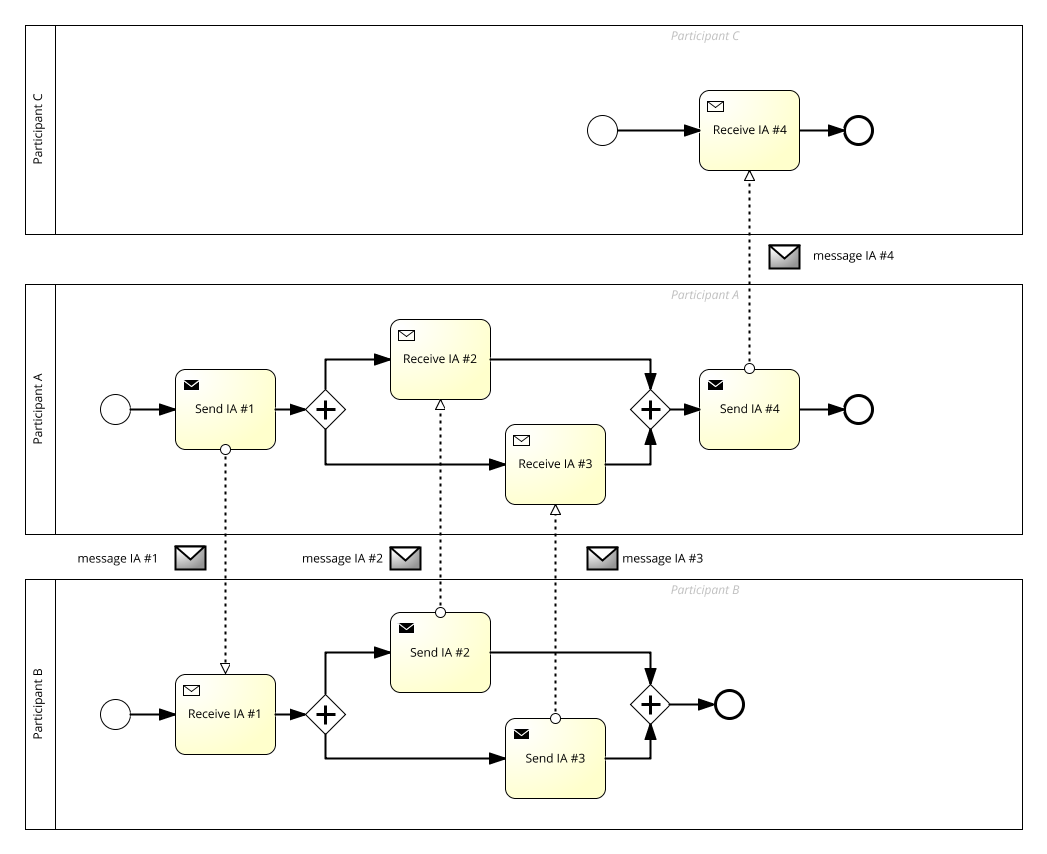
\includegraphics[width=1\textwidth]{src/images/collab2bpm.png}
\caption{BPMN/XML Translation Example - Collaboration Model}
\label{fig:collab2bpmn}
\end{figure}

The BPMN/XML shown in Example \ref{lst:collabbpmnex} represents the valid translation of the collaboration model shown in Figure \ref{fig:collab2bpmn}. Following the BPMN/XML convention, the root element is included as well the \textit{definitions} with the namespace and schema declarations. A layer below, the process independent data objects \textit{message}, the collaboration specific objects and a \textit{process} for each participant are defined. Within the \textit{collaboration} element, the participants, with a reference to their corresponding process and the message flow of the involving interacting tasks are declared. The \textit{messageFlow} object references the send and receive tasks that exchange the message. Or, if a process of a participant is represented as a black box, the \textit{messageFlow} object can also reference the process itself. In case of public or private models, where it is also possible that only one process of a specific participant is included, the \textit{messageFlow} object references the participant that sends or receives the message.

\lstset{language=XML, morekeywords={definitions, encoding, xmlns, typeLanguage, targetNamespace, xsi:schemaLocation, message, id, name, choreography, isClosed, participant, messageFlow, messageRef, sourceRef, targetRef, choreographyTask, initiatingParticipantRef, incoming, outgoing, participantRef, messageFlowRef, startEvent, endEvent, parallelGateway, exclusiveGateway, gatewayDirection, sequenceFlow, sendTask, receiveTask, task}, basicstyle=\tiny, breaklines=true, frame=single} 

\begin{lstlisting}[caption={BPMN Choreography Model Example},captionpos=b, label={lst:collabbpmnex}]
<?xml version="1.0" encoding="UTF-8"?>
<definitions xmlns="http://www.omg.org/spec/BPMN/20100524/MODEL" xmlns:xsi="http://www.w3.org/2001/XMLSchema-instance" typeLanguage="http://www.w3.org/2001/XMLSchema" xsi:schemaLocation="http://www.omg.org/spec/BPMN/20100524/MODEL http://www.omg.org/spec/BPMN/2.0/20100501/BPMN20.xsd">
   <message id="m1" name="message IA #1"/>
   <message id="m2" name="message IA #2"/>
   <message id="m3" name="message IA #3"/>
   <message id="m4" name="message IA #4"/>
   <collaboration id="collab1">
      <participant id="p1" name="Participant A" processRef="pr1"/>
      <participant id="p2" name="Participant B" processRef="pr2"/>
      <participant id="p3" name="Participant C" processRef="pr3"/>
      <messageFlow id="mf1" messageRef="m1" name="" sourceRef="t1" targetRef="t5"/>
      <messageFlow id="mf2" messageRef="m2" name="" sourceRef="t8" targetRef="t2"/>
      <messageFlow id="mf3" messageRef="m3" name="" sourceRef="t9" targetRef="t3"/>
      <messageFlow id="mf4" messageRef="m4" name="" sourceRef="t4" targetRef="pr3"/>
   </collaboration>
   <process id="pr1" name="Participant A">
      <sendTask id="t1" name="Send IA #1">
         <incoming>sf1</incoming>
         <outgoing>sf2</outgoing>
      </sendTask>
      <startEvent id="e1" name="start">
         <outgoing>sf1</outgoing>
      </startEvent>
      <parallelGateway gatewayDirection="Diverging" id="g1" name="AND1">
         <incoming>sf2</incoming>
         <outgoing>sf3</outgoing>
         <outgoing>sf4</outgoing>
      </parallelGateway>
      <receiveTask id="t2" name="Receive IA #2">
         <incoming>sf3</incoming>
         <outgoing>sf5</outgoing>
      </receiveTask>
      <receiveTask id="t3" name="Receive IA #3">
         <incoming>sf4</incoming>
         <outgoing>sf6</outgoing>
      </receiveTask>
      <sendTask id="t4" name="Send IA #4">
         <incoming>sf7</incoming>
         <outgoing>sf8</outgoing>
      </sendTask>
      <parallelGateway gatewayDirection="Converging" id="g2" name="AND1_merge">
         <incoming>sf5</incoming>
         <incoming>sf6</incoming>
         <outgoing>sf7</outgoing>
      </parallelGateway>
      <endEvent id="e2" name="end">
         <incoming>sf8</incoming>
      </endEvent>
      <sequenceFlow id="sf1" name="" sourceRef="e1" targetRef="t1"/>
      <sequenceFlow id="sf2" name="" sourceRef="t1" targetRef="g1"/>
      <sequenceFlow id="sf3" name="" sourceRef="g1" targetRef="t2"/>
      <sequenceFlow id="sf4" name="" sourceRef="g1" targetRef="t3"/>
      <sequenceFlow id="sf5" name="" sourceRef="t2" targetRef="g2"/>
      <sequenceFlow id="sf6" name="" sourceRef="t3" targetRef="g2"/>
      <sequenceFlow id="sf7" name="" sourceRef="g2" targetRef="t4"/>
      <sequenceFlow id="sf8" name="" sourceRef="t4" targetRef="e2"/>
   </process>
   <process id="pr2" name="Participant B">
      <startEvent id="e3" name="start">
         <outgoing>sf9</outgoing>
      </startEvent>
      <receiveTask id="t5" name="Receive IA #1">
         <incoming>sf9</incoming>
         <outgoing>sf10</outgoing>
      </receiveTask>
      <parallelGateway gatewayDirection="Diverging" id="g3" name="AND1">
         <incoming>sf10</incoming>
         <outgoing>sf11</outgoing>
         <outgoing>sf12</outgoing>
      </parallelGateway>
      <sendTask id="t6" name="Send IA #2">
         <incoming>sf11</incoming>
         <outgoing>sf13</outgoing>
      </sendTask>
      <sendTask id="t7" name="Send IA #3">
         <incoming>sf12</incoming>
         <outgoing>sf14</outgoing>
      </sendTask>
      <parallelGateway gatewayDirection="Converging" id="g4" name="AND1_merge">
         <incoming>sf13</incoming>
         <incoming>sf14</incoming>
         <outgoing>sf15</outgoing>
      </parallelGateway>
      <endEvent id="e4" name="end">
         <incoming>sf15</incoming>
      </endEvent>
      <sequenceFlow id="sf9" name="" sourceRef="e3" targetRef="t5"/>
      <sequenceFlow id="sf10" name="" sourceRef="t5" targetRef="g3"/>
      <sequenceFlow id="sf11" name="" sourceRef="g3" targetRef="t6"/>
      <sequenceFlow id="sf12" name="" sourceRef="g3" targetRef="t7"/>
      <sequenceFlow id="sf13" name="" sourceRef="t6" targetRef="t8"/>
      <sequenceFlow id="sf14" name="" sourceRef="t7" targetRef="t9"/>
      <sequenceFlow id="sf15" name="" sourceRef="t8" targetRef="g4"/>
   </process>
   <process id="pr3" name="Participant C">
   	<startEvent id="e5" name="start">
         <outgoing>sf16</outgoing>
   	</startEvent>
   	<receiveTask id="t8" name="Receive IA #4">
     	   <incoming>sf16</incoming>
         <outgoing>sf17</outgoing>
     	</receiveTask>
   	<endEvent id="e5" name="end">
         <incoming>sf17</incoming>
     	</endEvent>
      <sequenceFlow id="sf16" name="" sourceRef="t9" targetRef="g4"/>
      <sequenceFlow id="sf17" name="" sourceRef="g4" targetRef="e4"/>
   </process>
</definitions>
\end{lstlisting}

\section{Conclusion}
In this chapter, the followed \textit{top-down approach} of how to build a process collaboration, starting with the choreography model and then deriving the public and private models from it, was explained. It was also shown how the random choreography model generation can be influenced by specifying various build parameters as well as by imposing pattern-based compliance rules. Furthermore, all necessary components for generating sound choreography models that satisfy the three levels of correctness were introduced by explaining the involved generation algorithms as well as by pointing out the necessity of the \textit{Model Tracking} component, in which the model is decomposed into splits, branches and nodes. Also, the indispensability of the thereby involved control flow logic, with it's status model for branches and the necessary functionality of calculating the exact proportion of interactions that are at free disposal and those that have already determined places within the evolving model or those that will be needed later by paths that will be created by not yet consumed gateways, were highlighted. The chapter was concluded by explaining how the internal model representation is translated to BPMN/XML. Thereby, the mapping of the internal components to the corresponding BPMN/XML elements was shown.
In the next chapter, it will be explained how the introduced components of the random process collaboration generator are implemented within the CRISP framework.